%% Allgemeine Definitionen
\documentclass{article} %% Bestimmt die allgemeine Formatierung der Abgabe.
%\usepackage{a4wide} %% Papierformat: A4.
\usepackage[utf8]{inputenc} %% Datei wird im UTF-8 Format geschrieben.
%% Unter Windows werden Dateien je nach Editor nicht in diesem Format
%% gespeichert und Umlaute werden dann nicht richtig erkannt.
%% Versucht in diesem Fall "utf8" auf "latin1" (ISO 8859-1) wechseln.
\usepackage[T1]{fontenc} %% Format der Zeichen im erstellten PDF.
\usepackage[nswissgerman]{babel} %% Regeln für automatische Worttrennung.
\usepackage{fancyhdr} %% Paket um einen Header auf jeder Seite zu erstellen.
\usepackage{lastpage} %% Wird für "Seite X von Y" im Header benötigt.
                      %% Damit das funktioniert, muss pdflatex zweimal
                      %% aufgerufen werden.
\usepackage{enumerate} %% Hiermit kann der Stil der Aufzählungen
                       %% verändert werden (siehe unten).

\usepackage{amssymb} %% Definitionen für mathematische Symbole.
\usepackage{amsmath} %% Definitionen für mathematische Symbole.
\usepackage{tikz}  %% Paket für Grafiken (Graphen, Automaten, etc.)
\usetikzlibrary{arrows}   %% Tikz-Bibliothek für Pfeilspitzen
\usepackage{pgf-umlsd} %% Für das Sequenzdiagramm
\usepackage{pgf-umlcd} %% Für das Sequenzdiagramm 
\usepackage[font=small,labelfont=bf,tableposition=top]{caption}
\usepackage{paralist}
\usepackage{multicol}
\usepackage{lipsum}
\usepackage{mwe}

\renewcommand{\umlfillcolor}{white} %%Backgroundcolor for UML
\renewcommand{\umldrawcolor}{black} %%Bordercolor for UML


%% Quelle für Das Sequenzdiagramm: http://mirror.unl.edu/ctan/graphics/pgf/contrib/pgf-umlsd/pgf-umlsd-manual.pdf




%% Linke Seite des Headers
\lhead{\course\\\semester\\Projektbericht}
%% Rechte Seite des Headers
\rhead{\authorname\\Seite \thepage\ von \pageref{LastPage}}
%% Höhe des Headers
\usepackage[headheight=36pt]{geometry}
%% Seitenstil, der den Header verwendet.
\pagestyle{fancy}

\newcommand{\authorname}{Alexander Luyten\\Elias Arnold}
\newcommand{\semester}{Frühjahrssemester 2017}
\newcommand{\course}{Introduction to Internet and Security}

\title{OS-Fingerprinting Projektbericht\\
\begin{large}
Projekt zur Vorlesung: Introduction to Internet and Security
\end{large}}
\author{Alexander Luyten | Elias Arnold}


\begin{document}

\maketitle

\tableofcontents

\newpage

\section{Was ist OS-Fingerprinting}
Unter dem Begriff 'OS-Fingerprinting' versteht man das Erkennen des Betriebssystems, das von einem Zielhost verwendet wird. Um dies zu bewerkstelligen schaut man sich die Datenpakete dieses Hosts genauer an. Damit ein solches Packet das gewünschte Ziel erreichen kann und nicht irgendwo in den Tiefen des (heutzutage) riesigen Netzwerk von Netzwerken, dem Internet, verschwindet, müssen sich die Sender solcher Pakete an strenge Vorschriften halten. Eine ganze Palette von weiteren Informationen müssen in der richtigen Reihenfolge und Länge an die Nachricht angefügt werden (sog. "Header"). Der Inhalt einer Nachricht kann natürlich beliebig sein (In der Fachsprache "Payload" genannt). Man kann bei dem eben erklärten Prinzip Analogien zu vielen anderen Sender-/Empfänger-Prozessen erkennen. Zum Beispiel funktioniert die Briefpost nach einem ganz ähnlichen Prinzip. Der beliebige Inhalt eines Datenpaketes kann mit dem induviduellen Text im Nachrichtenfeld einer Postkarte verglichen werden. Die streng vorgeschrieben Mehrinformationen entsprechen hier der Angabe einer Empfängeradresse und dem Frankieren mit einer Briefmake genügenden Werts. Üblicherweise kann der Empfänger eines Briefes/Postkarte den Absender eindeutig indentifizieren, weil der Inhalt des Briefes vom Absender gekennzeichnet ist. Im Internet funktioniert das nicht. Fordert man ein Server dazu auf, einem Informationen zukommen zu lassen (z.B. durch Aufrufen einer Webseite), kann man zwar seine Adresse bestimmen, mit der er im Internet kommuniziert (mit Hilfe des DNS-Servers), jedoch kann man daraus keine Informationen über den Server selbst ableiten. Da dieser Server aber eine Antwort über das Internet an den Sender zurückschickt, muss auch er zusätzliche Informationan an die eigentliche Antwort anhängen. Diese Aufgabe wird von TCP/IP-Stack übernommen, der je nach Betriebssystem etwas anders aussieht, und dementsprechend leicht andere Pakete verschickt. Diese minimalen Unterschiede macht man sich beim OS-Fingerprinting zu Nutzen und versucht daraus trotzdem Rückschlüsse über den Server, insbesondere über das verwendete Betriebssystem, zu ziehen. Bei der Briefpost kann man das mit der Handschrift des Senders vergleichen, die zwar je nach Sender unterschiedlich ist, aber (falls leserlich geschrieben) trotzdem vom Empfänger gelesen werden kann. 

\begin{figure}[h]
\begin{center}
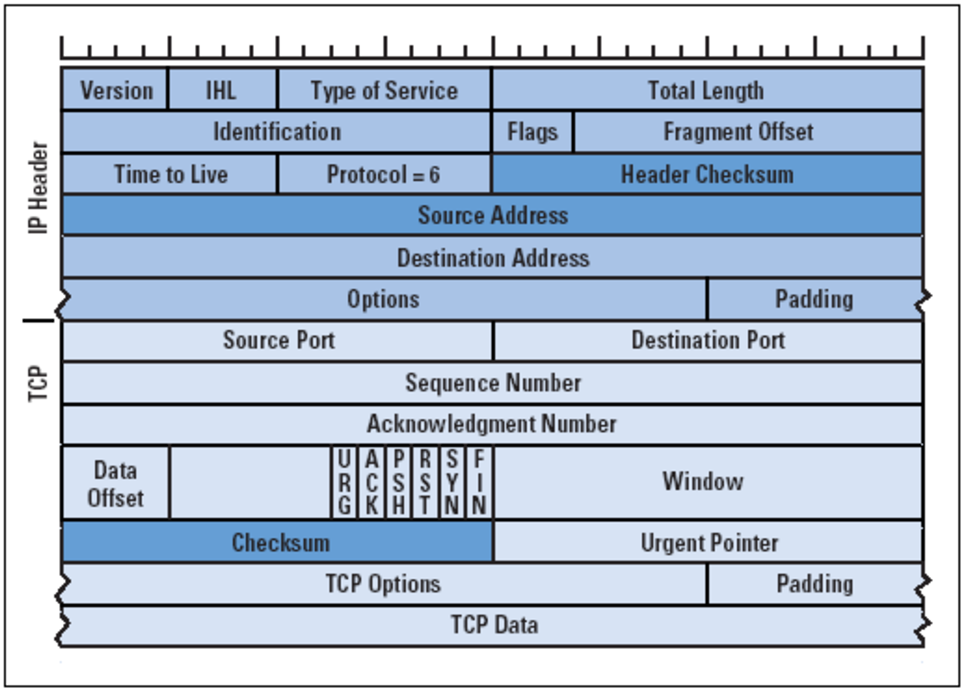
\includegraphics[width=0.5\textwidth]{data/grafik1.png}
\caption{Der IP-Header der bei jedem Datenpaket vorhanden sein muss. Sowie der TCP-Header, welcher für eine stabile Verbindung zwar benötigt, aber nicht zwingend vorhanden sein muss. \cite{tcpipstack}}
\label{Abbildung1}
\end{center}
\end{figure}


\newpage

\section{Warum OS-Fingerprinting?}
Wie im vorherigen Kapitel bereits erläutert, kann man durch gezieltes Auslesen der Headerinformationen von Paketen im Internet, Informationen über das Betriebssystem eines Senders gewinnen. Doch welchen Nutzen ergibt sich aus den Informationen, die man mittels OS-Fingerprinting gewinnt?
Der sicherheitsbewusste Leser wird nun gleich an einen massiven Einschnitt in die Privatsphäre sowie an Spionage denken. Den ersten Punkt, den Einschnitt in die Privatsphäre, kann man grösstenteils verwerfen, da der Markt nur eine begränzte Palette an Betriebssystemen bereitstellt, und nicht alle Menschen ein induviduelles, privates OS besitzen. Natürlich gibt es hier Ausnahmen. Jedoch muss die Person, die ihr Betriebssystem umkonfiguriert oder sogar komplett neu geschrieben hat, sehr weitreichende Informatikkenntnisse gehabt haben, und musste den Auswirkungen und Folgen Ihrer Tat vollumfänglich bewusst gewesen sein. Unter dem Strich benutzt jeder Mensch ein von Experten entwickeltes und OS, dem man mit OS-Fingerprinting keine persönlichen Informationen entlocken kann. Darum kann man hier nicht von einer Verletzung der Privatsphäre sprechen.\\
\\
Ein weiteres Vorurteil gegenüber OS-Fingerprinting stellt die Tatsache dar, dass es darum geht, das Verhalten eines Zielsystems auszuspionieren. Diesen Kritikpunkt kann man nicht abstreiten. Für Hacker ist dies eine wichtige Information, um ihre Shellskripte auf dem Zielrechner ausführen zu können \cite{nmap_osdetect}. Grosse Firmen heuern sogar Hacker (sog. Pentester) an, welche versuchen, in das Firmennetz einzudringen, um die eigene IT-Infrastruktur auf Herz und Nieren zu prüfen \cite{pentester}. Egal ob der Hacker böse oder gute Absichten hat, er braucht, um seine 'Arbeit' verrichten zu können, zuverlässige Informationen über das jeweilige Betriebssystem.\\
\\
Jedoch müssen die gewonnen Informationen nicht unbedingt dazu verwendet werden, leichter in ein fremdes System einzudringen. Manchmal reicht es völlig aus, zu wissen, welche Systeme im eigenen Netzwerk verwendet werden, oder ob diese das tun, was man von ihnen erwartet. So kann eine Firma zum Beispiel testen, ob alle Mitarbeiter mit der aktuellen Version eines Betriebssystems ausgerüstet sind und es bei ihnen reibungslos läuft.

\section{Methoden}
Alle Methoden, die für OS-Fingerprinting verwendet werden, funktionieren nach dem Prinzip, möglichst viele Informationen über Eigenheiten und Charakteristiken eines Zielsystems zu gewinnen, und diese nachher mit bereits bekannten Informationen über das Verhalten verschiedener Betriebssysteme zu vergleichen. Um das zu bewerkstelligen gibt es verschiedene Ansätze \cite{forensicswiki}. Dabei kann man die benötigten Informationen von Headern auslesen, die unterschiedlich Tief im TCP/IP-Stack an die Nachricht angefügt werden. Wir haben uns für Header Entschieden, die im Tranport- oder Network-Layer angefügt werden (TCP, ICMP,IP). Wenn man Pakete des Zielhosts auslesen will, dann unterscheident man zwischen zwei Methoden: Der Aktiven- und der Passiven-Methode. Beim aktiven OS-Fingerprinting generiert man Anfragepakete und verschickt diese an den Zielhost in der Hoffnung, darauf eine Antwort zu bekommen. Bei der passiven-Methode wird kein eigener 'traffic' verursacht, daher können nur Pakete des Zielhosts ausgelesen werden, wenn dieser aus irgendeinem Grund zu senden beginnt. Ein weiteres Unterscheidungsmerkmale der Aktiven Methode ist die Zuverlässigkeit. Man darf davon ausgehen, dass die induviduellen Anfragen vom Zielhost beatwortet werden, jedoch fällt man durch das aktive Senden viel eher auf, weshalb die Anonymität beeintrachtigt wird.

\section{Setup}

\subsection{Konfiguration}
Ziel des Projektes war es, selber ein Tool zu entwickeln, um OS-Fingerprinting zu betreiben. Die erste Frage die wir uns stellen mussten war, ob wir die Aktive- oder die Passive-Methode verwirklichen sollen. Da in absehbarer Zeit ein Resultät/eine Vermutung über das verwendete Betriebssystem vorliegen soll, haben wir uns für die zuverlässige, Aktive-Methode entschieden. Wie im obigen Kapitel 'Methoden' bereits betont, liegt der Vorteil dieser Methode nicht nur im aktiven Senden von Anfragen an den Zielhost, sondern auch in der induviduellen Gestaltung dieser Anfragepakete. \\
Zu Beginn des Projektes haben wir den Fokus weniger auf den Zusammenbau dieser 'Massgeschneiderten' Anfragen gelegt, sondern viel mehr auf den groben Ablauf eines Tests und die dafür notwendigen Klassen und Methoden. Dabei haben wir unsere Überlegungen mit der Programmiersprache Java in die Tat umgesetzt (Erstversuch). Wie die bereits existierenden Sniffer-Programme wollten auch wir das Pcap Interface implementieren. Unter Windows haben wir dazu die Bibliotheken WinPcap und jNetPcap (Java-Wrapper für WinPcap) verwendet. Das einbinden in Java war ein Kinderspiel \cite{jNetPcap-Tutorial}. Jedoch hatten wir erhebliche Schwierigkeiten, dasselbe unter Linux-Distributionen wie zum Beispiel Ubuntu zu tun, welhalb wir uns schlussendlich der Programmiersprache Python zuwendeten. Die Aussagekräftigsten Infomationen mit denen sich Rückschlüsse auf das verwendte Betriebssystem ziehen lassen, befinden sich im IP- und TCP-Header. In allen unseren Versuchen wollten wir  mit dem Zielsystem eine TCP-Verbindung aufbauen, um an diese Header zu kommen und daraus die aussagekräftigen Daten zu extrahieren.
\begin{figure}[!htb]
\begin{center}
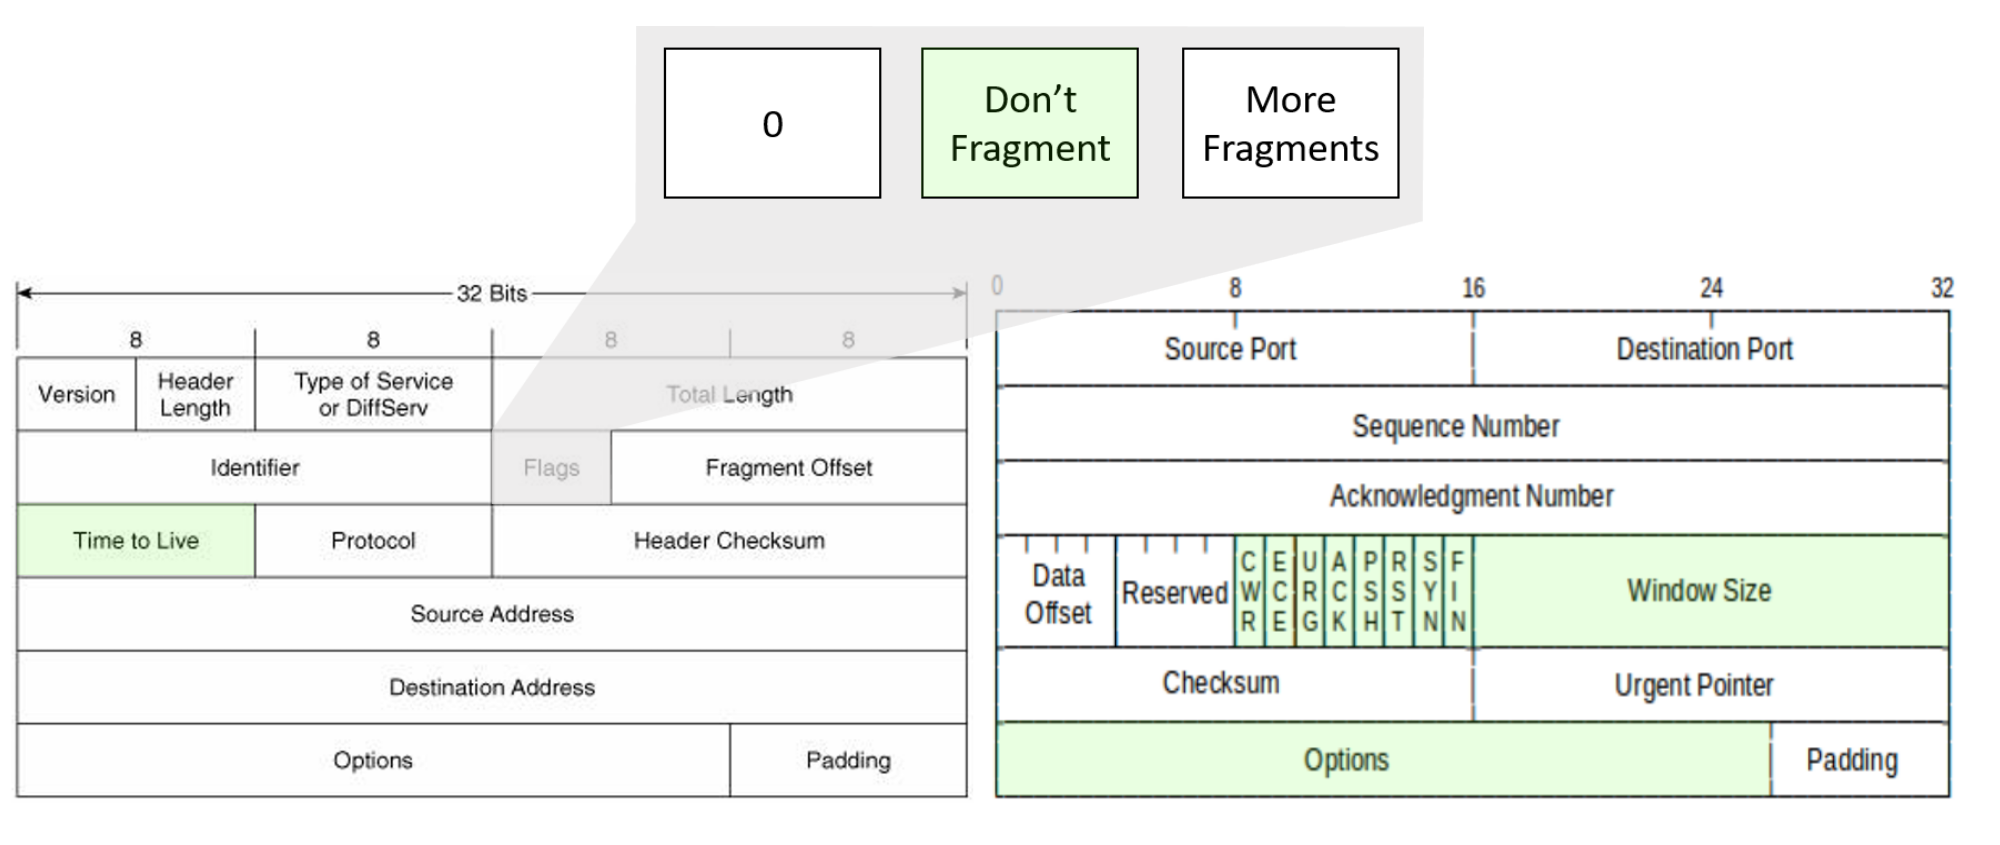
\includegraphics[width=0.9\textwidth]{data/grafik5.png}
\captionsetup{singlelinecheck=off}
\caption[Titel]{Der TCP-Header(rechts) und der IP-Header(links). Datenfelder sind in Hellgrün markiert: 
\normalfont
\begin{itemize}
\item Time to Live (TTL): Anzahl Hops die ein Paket maximal zurücklegen darf.
\item Don't Fragment: Ein Bit das festlegt, ob eine Nachricht in kleinere Stücke unterteilt werden darf. Je nach OS unterschiedlich bei kleineren Paketen.
\item TCP-Control-Flags: Diese Zustände werden benötigt, um wichtige Kontrollpakete zu kennzeichnen.  
\item Window Size: Anzahl der Pakete, die der Empfänger am Stück empfangen möchte
\item TCP-Options: Unterschiedlich grosse Zusatzinformationen
\end{itemize}
}%ende caption
\label{Abb.4}
\end{center}
\end{figure}

\subsection{Erstversuch}
Die erste Idee war, dem Zielhost ein simples ICMP-Ping-Paket zu schicken, sowie mit ihm eine TCP-Verbindung aufzubauen. Unabhängig davon ob die TCP-Verbindug zustande kommt (3-Wege-Handshake) oder nicht, werden so TCP-Header in beide Richtungen ausgetauscht. In Java blockt die '\texttt{connect()}'-Methode aber solange, bis die Verbindung aufgebaut oder abgelehnt wurde. Um dieses Problem zu umgehen, mussten wir mit Threads arbeiten, um gleichzeitig zum Verbindunsversuch die ausgetauschten Datenpakete abfangen zu können. Jedoch ergab sich durch die Arbeit mit Threads wiederum ein neues Problem: Da man nicht voraussagen konnte welcher Thread wie lange für den Verbindungsaufbau braucht, mussten wir die Ausgaben der einzelnen Threads in eine Datencontainer-Klasse umleiten, um sie nach den Tests geordnet ausgeben zu können. Ein Ablaufdiagramm sowie ein Screenshot unseres ersten Versuchs in Java finden Sie im Anhang (A.1 und A.2).\\


\section{Schutz vor OS Fingerprinting}
Wie im einleitenden Kapitel bereits angetönt, sind Informationen über das OS auf einem Zielrechner eine sehr wichtige Information für Hacker. So liegt natürlich der Gedanke nicht weit, mit kleinen Veränderungen am TCP/IP Stack potentiellen OS-Fingerprintern ein falsches Betriebssystem vorzugaukeln. Da jeder durch OS-Fingerprinting gewonnenen Information eine bestimmte Relevanz zugeordnet werden muss, reicht es meistens schon aus, einen Parameter des eigenen TCP/IP Stacks zu verändern. Unser Endprodukt verwendet einfache \texttt{if} Statements, um das Betriebssystem zu bestimmen. Liegen die erforderlichen Headerfelder erstmal vor, verwendet FingerBerry die TTL des IP-Headers (Dieses Feld ist in jedem Netzwerkpaket präsent) als erste Instanz, um die Suche zwichen den Bertriebssystemklassen  eizugränzen. Um sich jetzt vor OS-Fingerprinting zu schützen, oder zumindest um den Angreiffer in die Irre zu führen, ist eine Option die eigene TTL (Time to Live) zu verändern, die jedem Netzwerkpaket das den eigenen Host verlässt im IP-Header mitgegeben wird.\\
Diese Idee verfolgten wir mit unserem Tool: 'Faker' (Screenshot im Anhang A.3). Da FingerBerry auch nur auf Linuxartigen Betriebssystemen läuft, funktioniert der Faker auch nur auf Linux-Derivaten. Jedoch kann man das auch manuell machen, indem man (unter Linux) folgende Datei verändert:\\\texttt{~/proc/sys/net/ipv4/ip\_default\_ttl}. Auf Linux Betriebssystemen ist Standartmässig der TTL-Wert auf 64 gesetzt. Da diese Zahl aber bei jedem Hop zwischen Ihnen und dem OS-Fingerprinter um eins verringert wird, ist es eine schlechte Wahl, diesen wert nur gering zu verändern (z.B auf 63 zu setzen). Sie können diesen Wert natürlich frei wählen. Wollen Sie jedoch ein bestimmtes Betriebssystem simulieren, hilft ihnen folgende Liste weiter:
\begin{figure}[!h]
\begin{center}
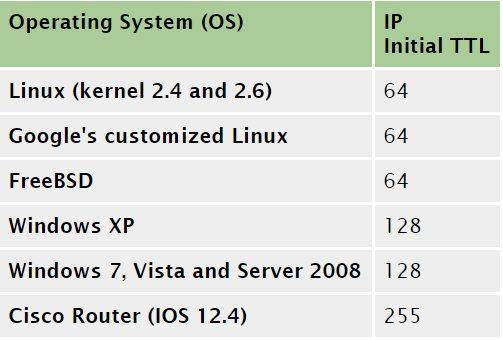
\includegraphics[scale=0.8]{data/grafik6.png}
\captionsetup{singlelinecheck=off}
\caption[Titel]{
Die Standard TTL Werte nach Betriebssystem \cite{default_ttl_list}
}%ende caption
\label{Abb.54}
\end{center}
\end{figure}
\newpage
\section{Resultate}
\subsection{Endprodukt}
Nach dem 'Fehltritt' mit Java, haben wir uns entschieden, mit Python weiter zu arbeiten. Unser Endprodukt tr\"{a}gt den Namen 'FingerBerry' und ist eine interaktive Konsolenanwendung.\\
Um die Applikation zu installieren, muss man die ben\"otigten Quelldateien herunterladen, ausserdem muss Python3 auf dem Computer installiert sein. Die Datei \texttt{Application.py} muss mit Administratorrechten ausgef\"uhrt werden, damit man die ben\"otigten Rechte bekommt, um die Netzwerkinterfaces abzuh\"oren und selber Raw Packets zu verschicken. \\
Nach Aufstarten der Applikation wird der Benutzer mit dem FingerBerry ASCII Logo begr\"{u}sst. Dem Benutzer stehen verschiedene Befehle zur Verf\"{u}gung. Falls man mit der Syntax nicht vertraut ist, gibt man einfach 'help' ein, und alle möglichen Befehle werden aufgelistet. Das sieht dann etwa wie folgt aus:
\begin{itemize}
	\item fingerprint <interface> <target-ip> -- guess of the target OS
	\item port <target-ip> <from portNr.> <to portNr.> -- performs a Portscan
	\item ip <interface> -- prints current ip of interface
	\item interfaces -- lists all Network-interfaces of your computer
\end{itemize}
Die grundlegende Funktionsweise von 'FingerBerry' ist stark an das Sequenzdiagramm im Anhang angelehnt. Jedoch geht unser Endprodukt weit über die dort vorgesehene Funktionalität hinaus. Ein UML-Klassendiagramm von 'FingerBerry' finden sie ebenfalls im Anhang (A.4). 
\newpage
%\begin{figure}[!htb]
%\begin{center}
%\includegraphics[width=0.9\textwidth]{data/FingerBerry_Info.png}
%\captionsetup{singlelinecheck=off}
%\caption{Eine Collage zweier Ausgaben von FingerBerry. Auf der linken- Seite ist die Intro-Grafik in ASCII-Art zu sehen. Auf der rechten- Seite  sieht man eine Zusammenfassung aller Testresultate.
%}%ende caption
%\label{Abb.54}
%\end{center}
%\end{figure}
\subsection{Probes}
Probes sind gef\"alschte TCP oder ICMP Packete, die dem Zielhost gesendet werden. Nach Versenden der verschiedenen Probes wartet man auf eine Antwort von dem Zielhost. Die Antwortpackete werden dann analysiert.\\
Verschiedene Betriebssysteme antworten anders auf die verschiedenen Probes. In der Regel sind die Probes nicht sinngem\"asse TCP oder ICMP Packete. In unserem FingerBerry Fingerprinting Tool verwenden wir drei verschiedene Probes: 
\begin{itemize}
	\item TCP Probe: Sinngem\"asses TCP Packet, dass dem Zielhost auf einem offenen Port gesendet wird. Dient ledlich zum Auslesen verschiedener Informationen, wie z.B. TTL, Window Size und andere TCP Optionen die gesetzt sind.
	\item ICMP Probe: Dient zum Auslesen der ICMP Optionen.
	\item FIN Probe: Ist ein nicht sinngem\"asses TCP Packet. Dem Zielhost wird ein TCP Packet gesendet mit dem FIN Bit gesetzt. Da keine Verbindung initialisiert wurde, also der 3-Way Handshake garnie stattgefunden hat sollte der Zielhost gem\"ass RFC 793 TCP ein Antwortpaket mit dem RST Bit gesetzt zur\"ucksenden. Was wirklich passiert, variiert von Betriebssystem zu Betriebssystem. Ein Screenshot des Probesenders finden sie im Anhang (A.5)
\end{itemize}
In unserer Applikation versenden wir zuerste eine FIN-Probe danach eine TCP- und eine ICMP-Probe. Danach evaluieren wir die Antwortpakete nach verschiedenen Eigenschaften.



\subsection{Packet Parser}
Ein Grossteil der Arbeit an unserer Applikation ging in das Auslesen der verschiedenen Antwortpakete, die wir vom Zielhost empfangen haben. Beim Auslesen der Daten hatten wir viele Schwierigkeiten, da wir nicht sehr gut vertraut waren mit dem TCP oder IP Header. Unsere Applikation liest die Antwortpakete als Bytes aus und interpretiert die verschiedenen Bytes anders. Dabei werden die verschiednen IP, TCP oder ICMP Header anders interpretiert. Die Bytes werden mit der Python \texttt{struct.unpack} Funktion in Datenformate umgewandelt, die man interpretieren kann, um das Betriebssystem zu erkennen. Ein Screenshot davon finden sie im Anhang (A.6).



\subsection{Interpretation der Informationen}
Nach Versenden von ICMP-/TCP-/FIN-Probes und Empfangen von Antwortpaketen k\"onnen wir alle erhaltenen Informationen interpretieren. F\"ur die Erkennung der verschiedenen Betriebssysteme haben wir am meisten Gewicht auf die Time to Live Headerinformation gesetzt. Diese Informationen haben uns am einfachsten eine Grobeinteilung der gr\"ossten Betriebssysteme gegeben und sind f\"ur praktisch alle Betriebssysteme per Default gleich gesetzt. Nach dem wir eine Grobeinteilung von Linux, Mac OS und Windows erhalten, unterteilen wir diese Betriebssysteme weiter, indem wir die Window Size betrachten. Dies erm\"oglicht es uns verschiedene Windows Betriebssysteme zu unterscheiden. \\
Zwischen Mac OS und Linux entscheiden wir, indem wir betrachten, ob eine Antwort erhalten wurde von der FIN-Probe oder nicht. \\

 
\subsection{Resultate}
Unser Fingerprinting Tool haben wir innerhalb dem Uni-Netzwerk an verschiedenen Zielhosts getestet. Die Resultate, die wir bekamen, waren ziemlich erfreulich. Bei 11 Zielsystemen haben wir 9 von 11 richtig erkannt. Dies entspricht einer richtigen Zuordnung von fast 80\%.\\
Was jedoch zu beachten ist, dass unsere Applikation nur die grossen Betriebssysteme: Linux, Mac OS, Cisco IOS, Windows 2000, Windows XP, Windows 7 und h\"oher unterscheiden kann. Dies ist in der Praxis nicht allzu n\"utzlich, da man mehr Informationen erhalten will \"uber die genaue Version des Betriebssystems, aber unsere Applikation macht eine zuverl\"assige Grobunterteilung der verschiedenen Betriebssystemen.

\begin{figure}[!htb]
\begin{center}
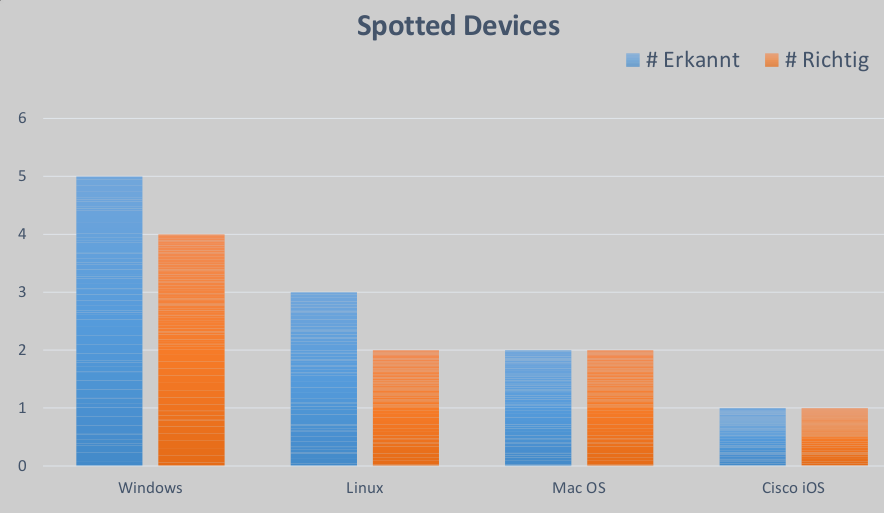
\includegraphics[width=0.8\textwidth]{data/spotteddevices.png}
\captionsetup{singlelinecheck=off}
\label{Abb.54}
\end{center}
\end{figure}


%\begin{enumerate}
%\item Vorstellung von Finger-Berry
%\item Installationshinweise, sonstige Informationen zum Tool
%\item Beschreibung der einzelnen Probes
%\item Vorstellen des Netzwerkpacket-Parsers (Empfängers)
%\item Finger Berry Testresultate (Grafik)
%\end{enumerate}
\newpage
\subsection{Lessons Learned}
Wärend der Arbeit am Projekt haben wir viel über die einzelnen Header und den Sinn und Zweck ihrer Felder gelernt. Die verschiedenen Optionen des TCP-Headers haben unser Interesse besonders geweckt. An dieser Stelle möchten wir ihnen kurz die 'Window-Scale-Option' vorstellen:\\
\\
Die 'Window-Scale-Option' ist, wie der Name schon vermuten lässt, eine optionale Zusatzinfomation für den TCP-Header. Im standartisierten Teil dieses Headers mit fixer Länge (20 Bytes), ist im 'Window-Size' Feld bereits angegeben, wie gross das Empfangsfenster (Menge an Daten die empfangen werden können, ohne deren Erhalt dem Sender zu bestätigen) gewählt werden soll. Da sich im Laufe der Zeit die Übertragunstechniken stets verbessert haben (wenige Bitfehler) und vor allem viel schneller geworden sind, muss das Empfangsfenster vergrössert werden, da es sonst viel zu wenig ausgelastet ist. Diese Aufgabe probiert die 'Window-Scale-Option' zu lösen:

\begin{figure}[!htb]
\begin{center}
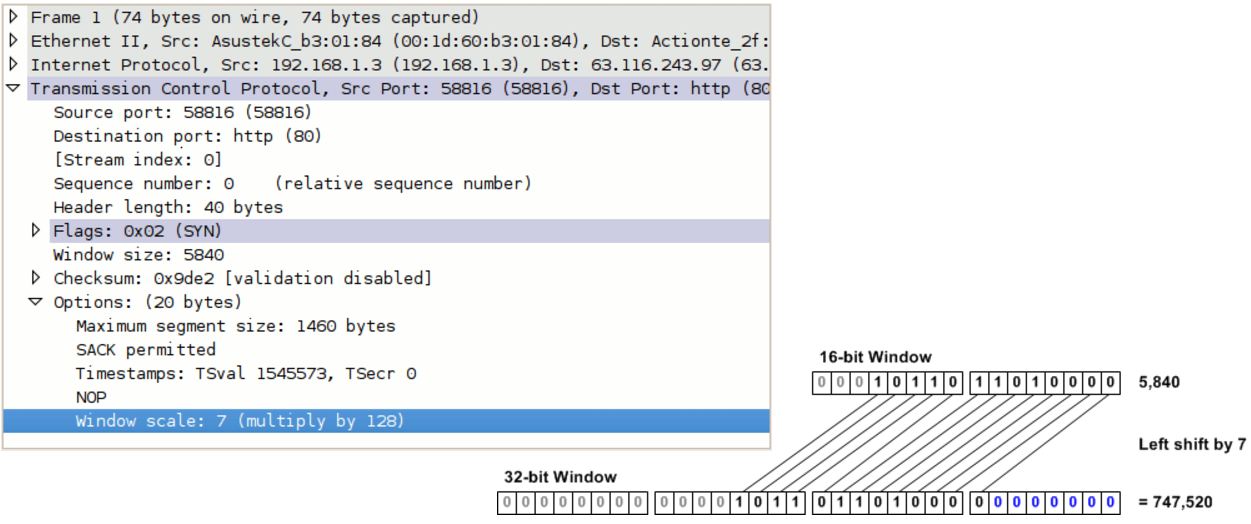
\includegraphics[width=0.9\textwidth]{data/grafik8.png}
\captionsetup{singlelinecheck=off}
\caption[Titel]{
Ein Screenshot aus Wireshark (links), sowie eine illustrative Grafik der Veränderung der Empfangsfenstergrösse mittel Bitshifting um sieben Bits nach links (Entspricht Multiplikation mit $2^7=128$) \cite{packetlife}. 
}%ende caption
\label{Abb.54}
\end{center}
\end{figure}

Während des Projektverlaufs mussten wir uns insbesondere mit Kommunikationsprolemen innerhalb des Teams herumschlagen. Wir hätten uns den ganzen Aufwand der mit dem wechseln der Programmiersprache oder dem Starten eines neuen Versuches sparen können, wenn wir uns in der Gruppe besser abesprochen hätten. Wir arbeiteten einfach drauflos, ohne sich vorher mit dem Teammitglied über das Vorhaben auszutauschen. Wenn wir das Projekt nochmals machen könnten, würden wir uns zuerst über die Ziele des Projekts und die Vorgehensweise Gedanken machen, und erst dann mit dem Code-Schreiben beginnen.\\
\\
Jedoch gab es aber auch die technischen Probleme, mit denen wir konfrontiert wurden. Beispielsweise gestaltete sich das Auslesen der Control-Flags als ziemlich anspruchsvoll, da in dem Bit-Array das die Zustände der Flags repräsentiert, auch führende Nullen eine Bedeutung haben. Python schneidet diese Nullen weg, wodurch sich das Ausledsen des restlichen Headers als extrem schwierig gestaltet. Die Lösung diesess Problems war Python-Methode \texttt{zfill()}, die ein Array bis zu einer gewünschten Länge mit Nullen auffüllt (Bei uns \texttt{zfill(8)} (8 Bit = 1 Byte)).

\newpage


%% Für mehr Beispiele - https://www.sharelatex.com/learn/Bibliography_management_with_bibtex
\begin{thebibliography}{9}
%\bibitem{latexcompanion} 
%Michel Goossens, Frank Mittelbach, and Alexander Samarin. 
%\textit{The \LaTeX\ Companion}. 
%Addison-Wesley, Reading, Massachusetts, 1993.
 
%\bibitem{einstein} 
%Albert Einstein. 
%\textit{Zur Elektrodynamik bewegter K{\"o}rper}. (German) 
%[\textit{On the electrodynamics of moving bodies}]. 
%Annalen der Physik, 322(10):891–921, 1905.
 
\bibitem{tcpipstack} 
Erle Robotics S.L:
\\\texttt{https://erlerobotics.gitbooks.io/erle-robotics-introduction-to-linux-networking/content\\/introduction\_to\_network/tcp\_and\_packets.html}

\bibitem{nmap_osdetect} 
Gordon Lyon, NMAP Network Scanning, Reasons for OS Detection:
\\\texttt{https://nmap.org/book/osdetect.html\#osdetect-reasons}(Stand: 12.06.2017)

\bibitem{pentester} 
Handelsblatt GmbH -\
ein Unternehmen der Verlagsgruppe Handelsblatt GmbH \& Co. KG
\\\texttt{http://www.wiwo.de/erfolg/trends/it-sicherheit-wo-hacker\\-ihr-unheimliches-handwerk-lernen-seite-4/5156098-4.html}(Stand: 12.06.2017)

\bibitem{forensicswiki} 
Forensicswiki - OS-Fingerprinting
\\\texttt{http://forensicswiki.org/wiki/OS\_fingerprinting}(Stand: 12.06.2017)
\bibitem{nmap_version_detection} 
Gordon Lyon, NMAP Network Scanning, Service and Version Detection:
\\\texttt{https://nmap.org/book/man-version-detection.html}(Stand: 12.06.2017)

\bibitem{nmap_wikipedia} 
wikipedia.org - nmap:
\\\texttt{https://de.wikipedia.org/wiki/Nmap}(Stand: 12.06.2017)

\bibitem{nmap_port_scanning_basics} 
Gordon Lyon, NMAP Network Scanning, Port Scanning Basics:
\\\texttt{https://nmap.org/book/man-port-scanning-basics.html}(Stand: 12.06.2017)

\bibitem{jNetPcap-Tutorial} 
Capturing network packets using jNetPcap API:
\\\texttt{https://compscipleslab.wordpress.com/2013/02/17/capturing-network-packets-through-java/}\\(Stand: 24.06.2017)

\bibitem{default_ttl_list} 
Common TTL Values by Netresec:
\\\texttt{http://www.netresec.com/?page=Blog\&month=2011-11\&post=Passive-OS-Fingerprinting}(Stand: 25.06.2017)

\bibitem{packetlife} 
Jeremy Stretch - TCP Windows and Window Scaling:
\\\texttt{http://packetlife.net/blog/2010/aug/4/tcp-windows-and-window-scaling/}(Stand: 28.06.2017)

\end{thebibliography}
\newpage

\appendix
\section{Anhang}
\subsection{Screenshot erster Versuch}
\begin{figure}[!htb]
\begin{center}
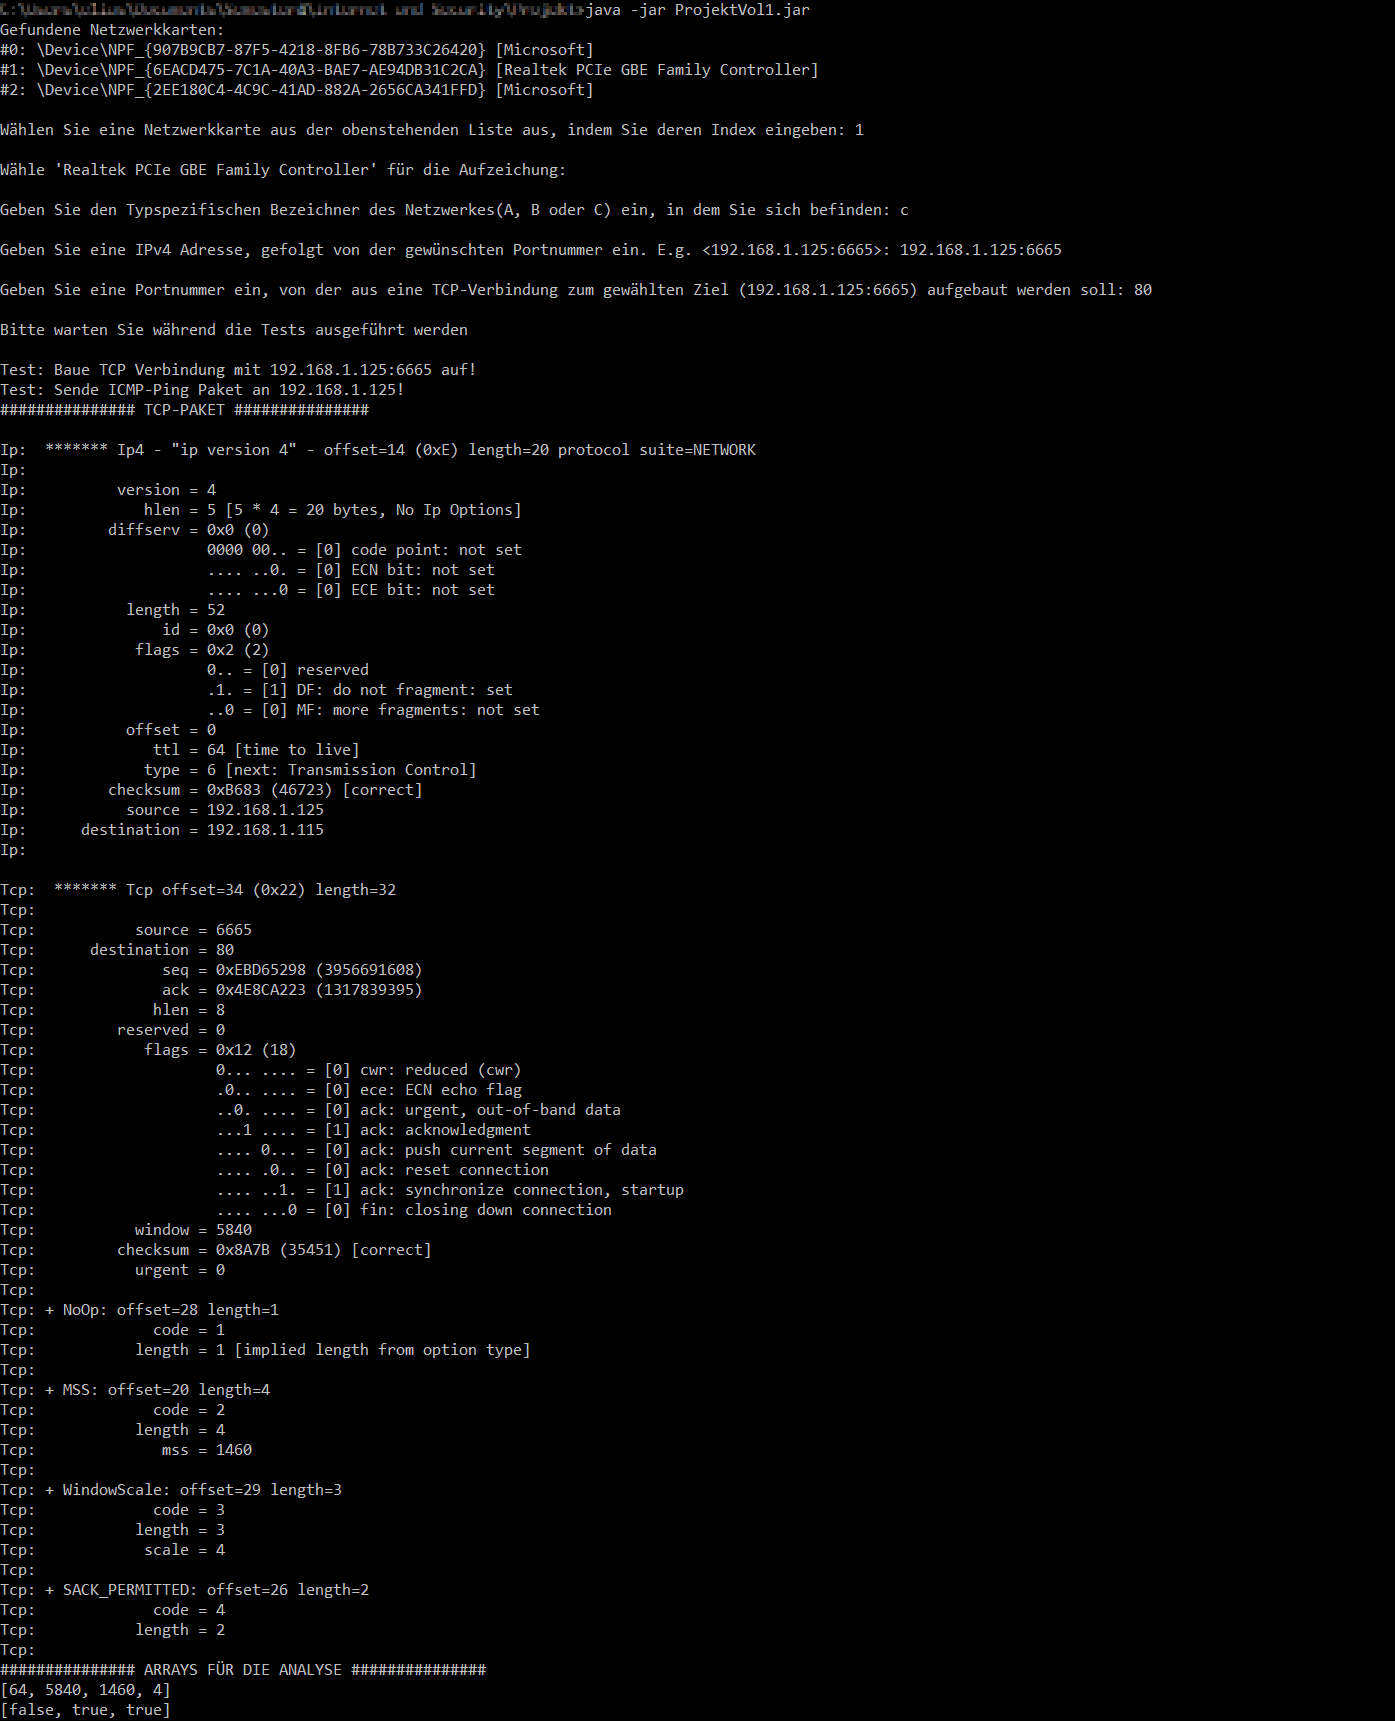
\includegraphics[height=0.5\paperheight]{data/grafik7.png}
\captionsetup{singlelinecheck=off}
\caption[Titel]{
Die Ausgabe unseres ersten Versuches mit Java. Das Bild zeigt lediglich den TCP-Test. Daneben wurde auch noch eine Ping Anfrage an den Zielhost geschickt (hier nicht im Bild). Man konnte jedes Byte des Antwortpaktes einzeln ansprechen und dessen Inhalt auslesen. Im obigen Bild wurde jede Information aus dem TCP-Paket (IP- und TCP-Header) ausgelesen und in einer Liste aufgeführt.
}%ende caption
\label{Abb.54}
\end{center}
\end{figure}
\newpage
\subsection{Sequenzdiagramm erster Versuch}
\begin{figure}[!htb]
  \begin{sequencediagram}
    \newthread{rec}{Receiver}
    \newinst[5]{con}{Container}
    \newinst{icmp}{ICMP-Sender}
    \newinst{tcp}{TCP-Sender}
    
    \begin{call}[2]{rec}{askForTarget()}{rec}{IP\&Port}
	\end{call}
	\postlevel
	\begin{call}[2]{rec}{askForMask()}{rec}{SubnetMask}
	\end{call}
	\postlevel
	\begin{messcall}[12]{rec}{new Container(Input)}{con}
	\end{messcall}
	\prelevel\prelevel\prelevel\prelevel\prelevel\prelevel\prelevel\prelevel\prelevel\prelevel\prelevel\prelevel
	\begin{sdblock}{sendProbes}{}
		\prelevel
		\setthreadbias{west}
		\begin{messcall}[2]{rec}{sendProbes()}{con}
		\end{messcall}
		\prelevel\prelevel\prelevel
		\begin{call}[2]{con}{}{icmp}{log()}
		\end{call}
		\prelevel\prelevel
		\begin{call}[2]{con}{}{tcp}{log()}
		\end{call}
		\prelevel
	\end{sdblock}
	\begin{sdblock}{ReceiveLoop}{}
		\prelevel
		\setthreadbias{west}
		\begin{messcall}{rec}{icmpresult()}{con}
		\end{messcall}
		\prelevel
		\begin{messcall}{rec}{tcpResult()}{con}
		\end{messcall}
	\end{sdblock}
	\begin{call}{rec}{getResult()}{con}{PrintableResult}
	\end{call}
  \end{sequencediagram}
  \caption{Das Sequenzdiagramm für den ersten Versuch. Dieses Konzept ist aber (bis auf kleine Änderungen) auch für die weiteren Versuche verwendet worden.}
\end{figure}
\newpage
\subsection{Screenshot des Fakers}
\begin{figure}[!htb]
\begin{center}
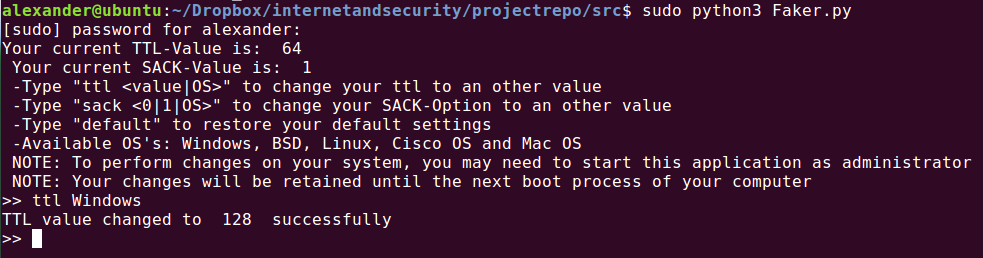
\includegraphics[width=0.9\textwidth, height=50mm]{data/faker.png}
\captionsetup{singlelinecheck=off}
\caption[Titel]{
Ein Screenshot von dem Fingerprint Faker. In der Abbildung wird die TTL auf den Windows Default-Wert gesetzt.  
}%ende caption
\label{Abb.54}
\end{center}
\end{figure}
\subsection{UML-Klassendiagramm von FingerBerry}
\begin{tikzpicture}%[show background grid]
\begin{class}[text width=7cm]{Application}{0,0} 
\attribute{running} 
\attribute{interfaces}
\operation{run(self):void}
\operation{run\_commsnd(self,command):void}
\operation{scan\_ports(interface,trget\_ip,from,to):void}
\operation{intro():void}
\operation[0]{help(command='NONE'):void}
\end{class}

\begin{object}[text width=7cm]{NetworkUtils}{9,0} 
\instanceOf{Abstract} 
\operation{get\_interfaces():String}
\operation{signal\_handler(self,signum,frame):Exception}
\operation{full\_port\_scan(source\_ip,target\_ip,\\source\_port,target\_port):void}
\operation{half\_port\_scan(source\_ip,target\_ip,\\source\_port,target\_port):void}
\operation{find\_open\_ports(source\_ip,\\target\_ip):Integer}
\operation{checksum\_tcp(msg):[Bit]}
\operation{get\_ip\_from\_hostname(interface,\\address):String}
\operation{get\_ip(interface):String}
\operation{checksum\_icmp(msg):[Bit]}
\end{object}

\begin{class}[text width=5cm]{FingerPrint}{0,-7} 
\attribute{mode} 
\attribute{source\_port}
\attribute{source\_ip}
\attribute{interface}
\attribute{target\_ip}
\attribute{target\_port}    
\operation{execute\_tests(self):void}
\operation{execute\_test(self,probe):[String]}
\operation{create\_table(self,results):void}
\operation{analyze(self,result):String}
\end{class}

\begin{object}[text width=4cm]{ProbeSender}{7,-9.5} 
\instanceOf{Thread} 
\attribute{probe} 
\attribute{interface}    
\operation{run(self):void}
\operation{change\_probe(probe):void}
\end{object}


\begin{object}[text width=4cm]{ProbeReceiver}{11,-7} 
\instanceOf{Thread} 
\attribute{probe} 
\attribute{interface}    
\operation{run(self):void}
\end{object}


\begin{abstractclass}[text width=5cm]{Probe}{11,-13} 
\attribute{source\_ip} 
\attribute{source\_port}
\attribute{target\_ip}
\attribute{target\_port}
\operation{send(self,target\_ip):void} 
\operation{receive(self):void} 
\end{abstractclass}

\begin{class}{TCP-Probe}{5,-13} 
\implement{Probe}  
\end{class}

\begin{class}{ICMP-Probe}{5,-15} 
\implement{Probe}  
\end{class}

\begin{class}{FIN-Probe}{5,-17} 
\implement{Probe}  
\end{class}
 


\association{NetworkUtils}{}{}{Application}{}{}
\association{FingerPrint}{}{}{Application}{}{}
\association{FingerPrint}{}{}{ProbeReceiver}{}{}
\association{FingerPrint}{}{}{ProbeSender}{}{}
\association{Probe}{}{}{ProbeSender}{}{}
\association{Probe}{}{}{ProbeReceiver}{}{}

\end{tikzpicture}
\subsection{Screenshot des Probesenders}
\begin{figure}[!htb]
\begin{center}
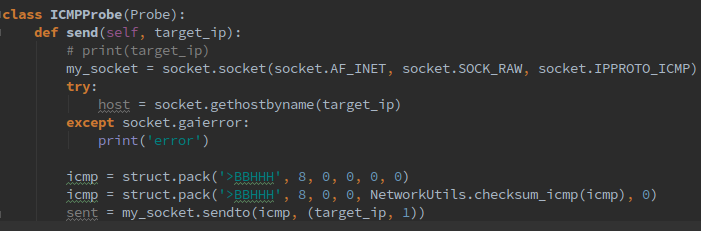
\includegraphics[width=0.9\textwidth]{data/probesend.png}
\captionsetup{singlelinecheck=off}
\caption[Titel]{
Ein Screenshot von der ICMPProbe Klasse. Die \texttt{send} Methode, ist zust\"andig fuer die Erstellung eines Raw Sockets und dem Versand des ICMP Packets. 
}%ende caption
\label{Abb.54}
\end{center}
\end{figure}
\subsection{Screenshot des Parsers}
\begin{figure}[!htb]
\begin{center}
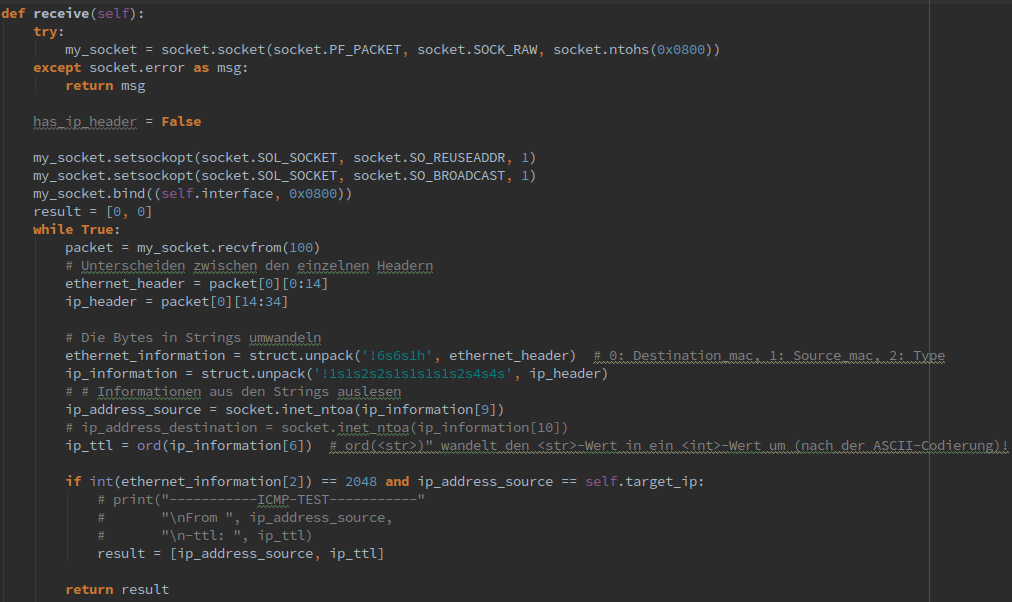
\includegraphics[width=0.9\textwidth]{data/probereceiver.png}
\captionsetup{singlelinecheck=off}
\caption[Titel]{
Ein Screenshot von der ICMP Klasse. Die \texttt{receive} Methode erstellt zuerst einen Raw Socket und empfangt Pakete auf diesenm. Diese Pakete werden mit \texttt{struct.unpack} entpackt und anschliessend wird \"uberpr\"uft, ob \"uberhaupt das gew\"unschte Paket empfangen wurde. Anschliessend werden die relevanten Informationen weitergegeben.
}%ende caption
\label{Abb.54}
\end{center}
\end{figure}
\end{document}